%\newsection{Kapitel1}

%Hier den Inhalt mit \input einfügen und die folgenden Zeilen entfernen



\section{Einleitung}

\s{% nur im Skript
Elektrische Bauelemente lassen sich in verschiedene Kategorien unterteilen, je nach ihrer Funktion und Arbeitsweise. 
Es gibt Widerstände, Kondensatoren, Spulen, aber auch Dioden und Transistoren, auf welche in einem späteren Kapitel eingegangen wird. 
Elektrische Bauelemente müssen über eine Quelle (Strom- oder Spannungsquelle) mit Energie versorgt werden, um ihre gewünschte Funktion zu erzielen.
Abbildung \ref{fig:Bauelemente} zeigt verschiedene Bauelemente.
\\

%%%%%%%%%%%%%%%%%%%%%%%%%%%%%%%%%%%%%%%%%%%%% Anfang - Abbildung Bauelemente %%%%%%%%%%%%%%%%%%%%%%%%%%%%%%%%%%%%
    \begin{figure}[h]
	\centering
		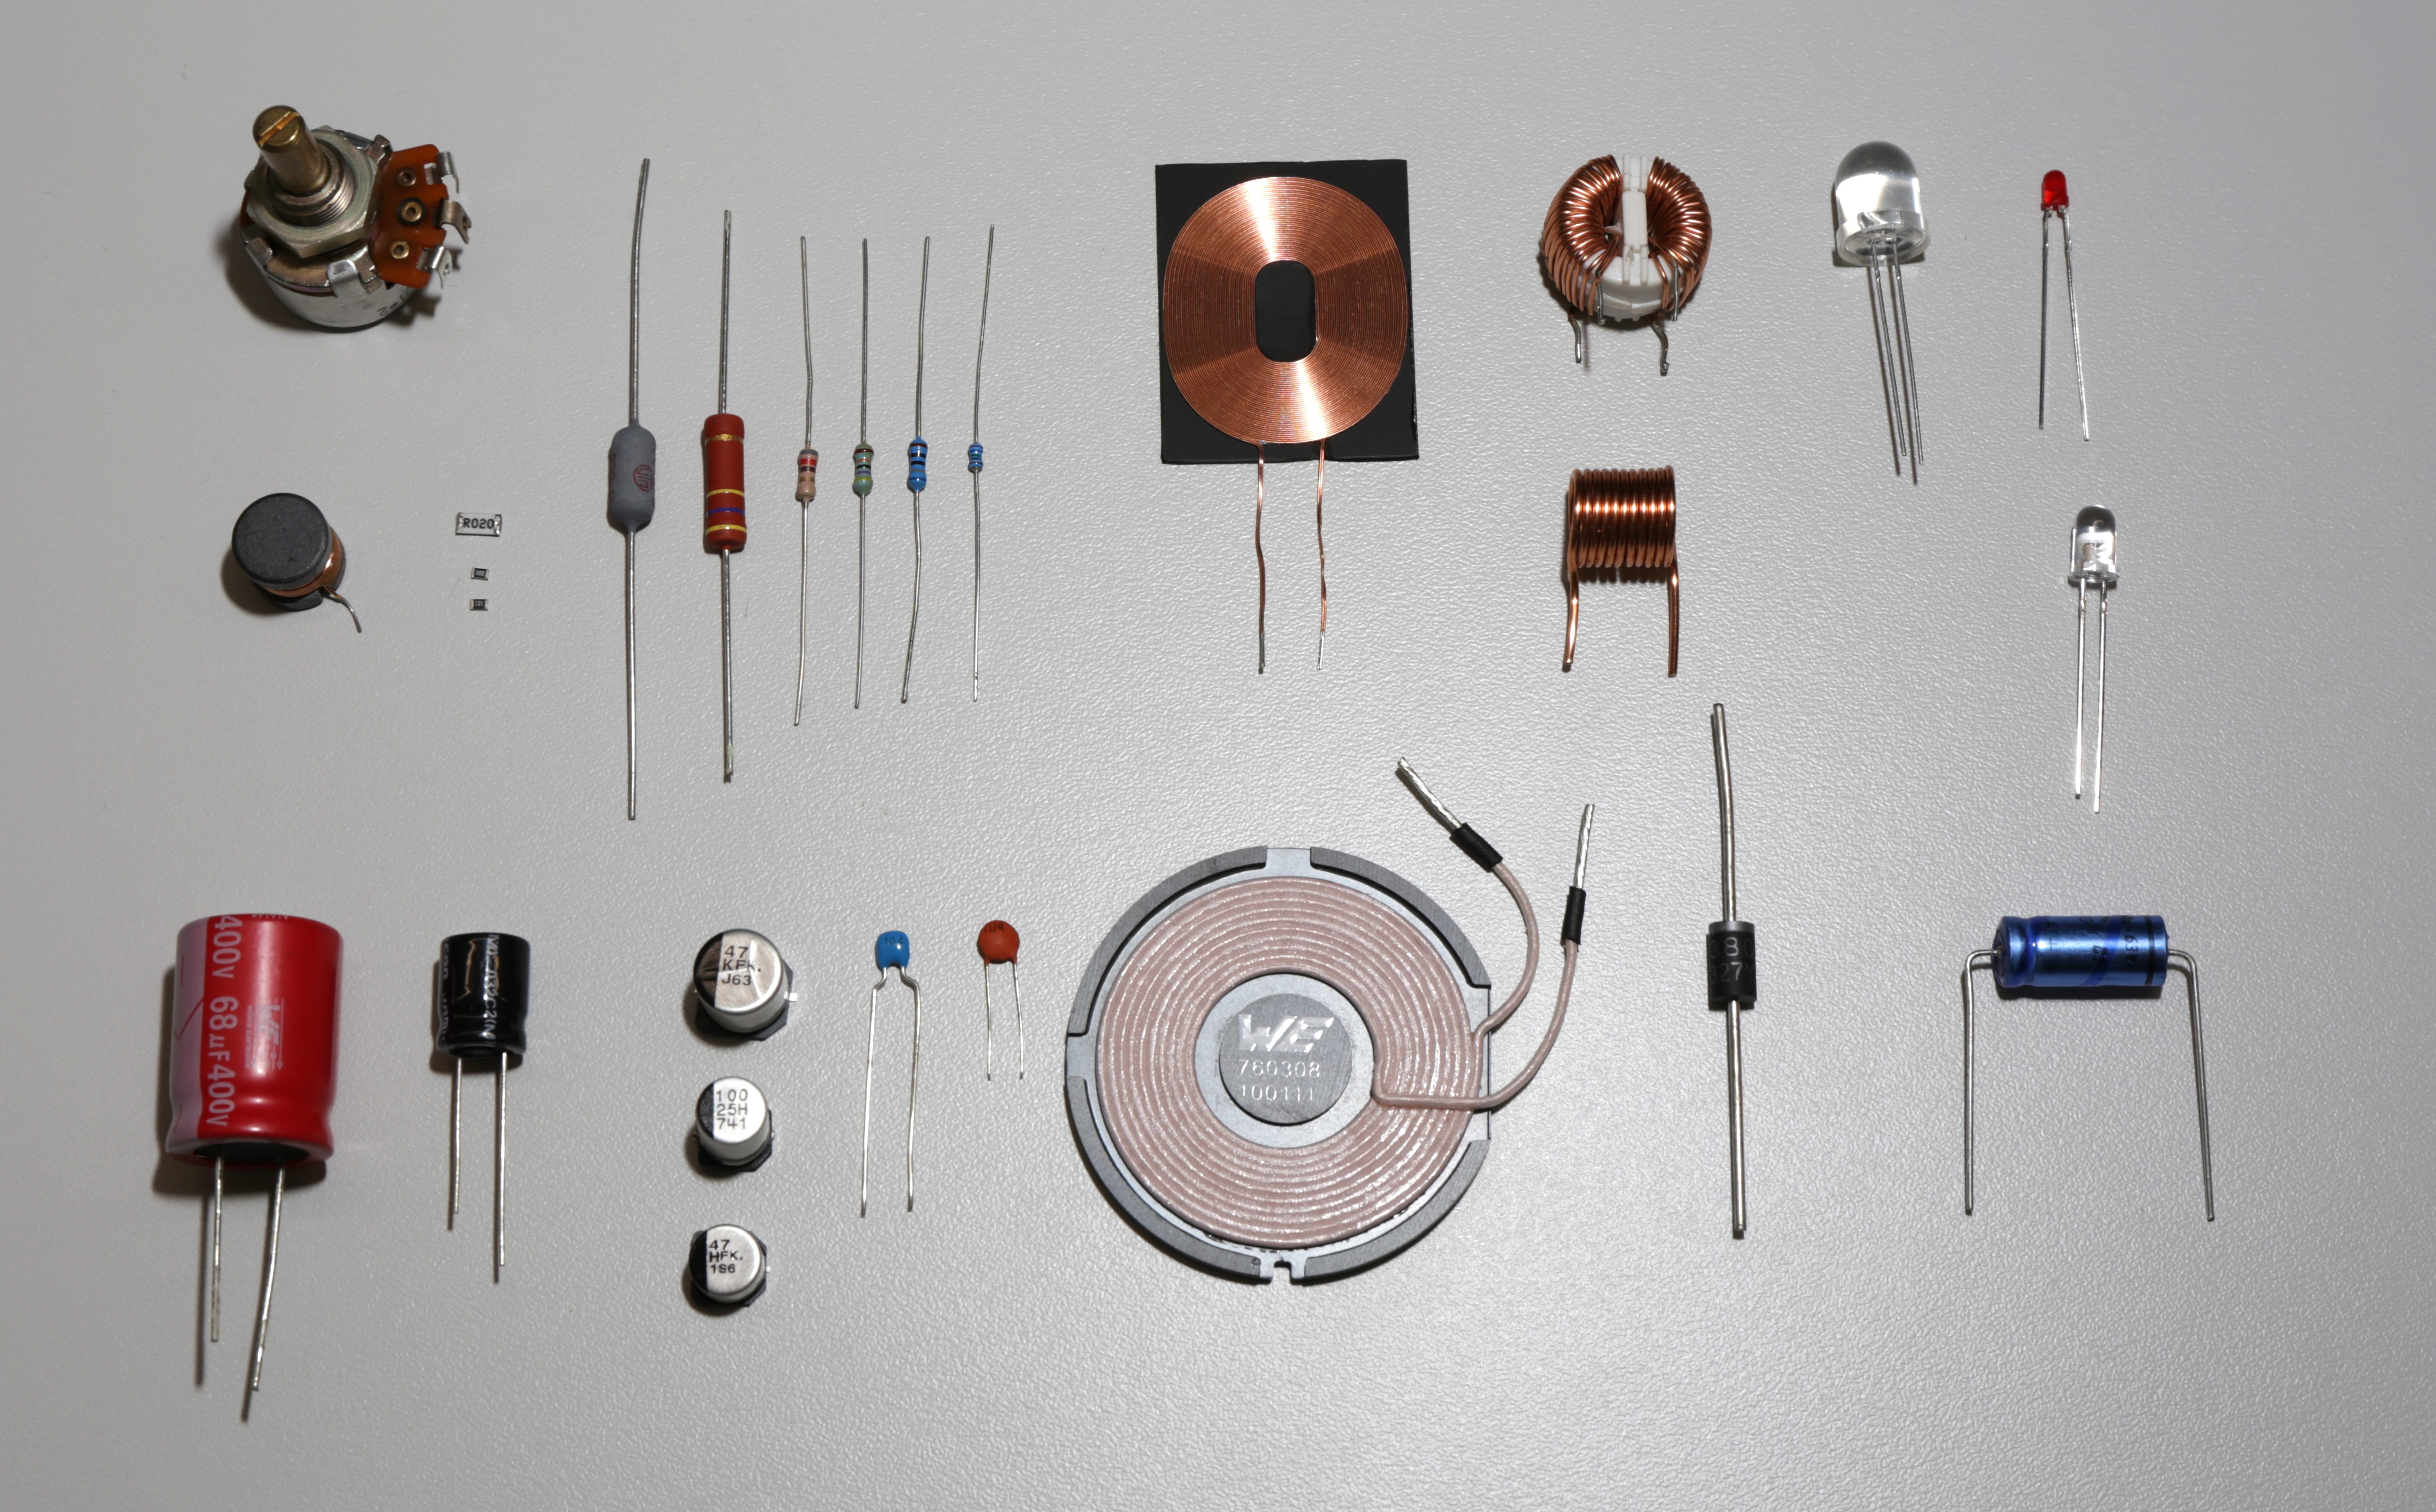
\includegraphics[width=0.8\textwidth]{ba}  
		\caption{\textbf{Verschiedene elektrische Bau­elemnte.} Zeigt elektrische Bauelemnte die in Schaltungen verwendet werden, wie Widerstände,
		 Kondensatoren, Spulen und Halbleiterbauelemente. Jedes Bauelement hat spezifische Eigenschaften und Funktionen zur Steuerung von Strom
		  und Spannung in einem elektrischen Netzwerk.}
		\label{fig:Bauelemente}
	\end{figure}
}% nur im Skript
\begin{frame}
	\ftx{Elektrische Bauelemente}
\b{
\begin{figure}[h]
	\centering
		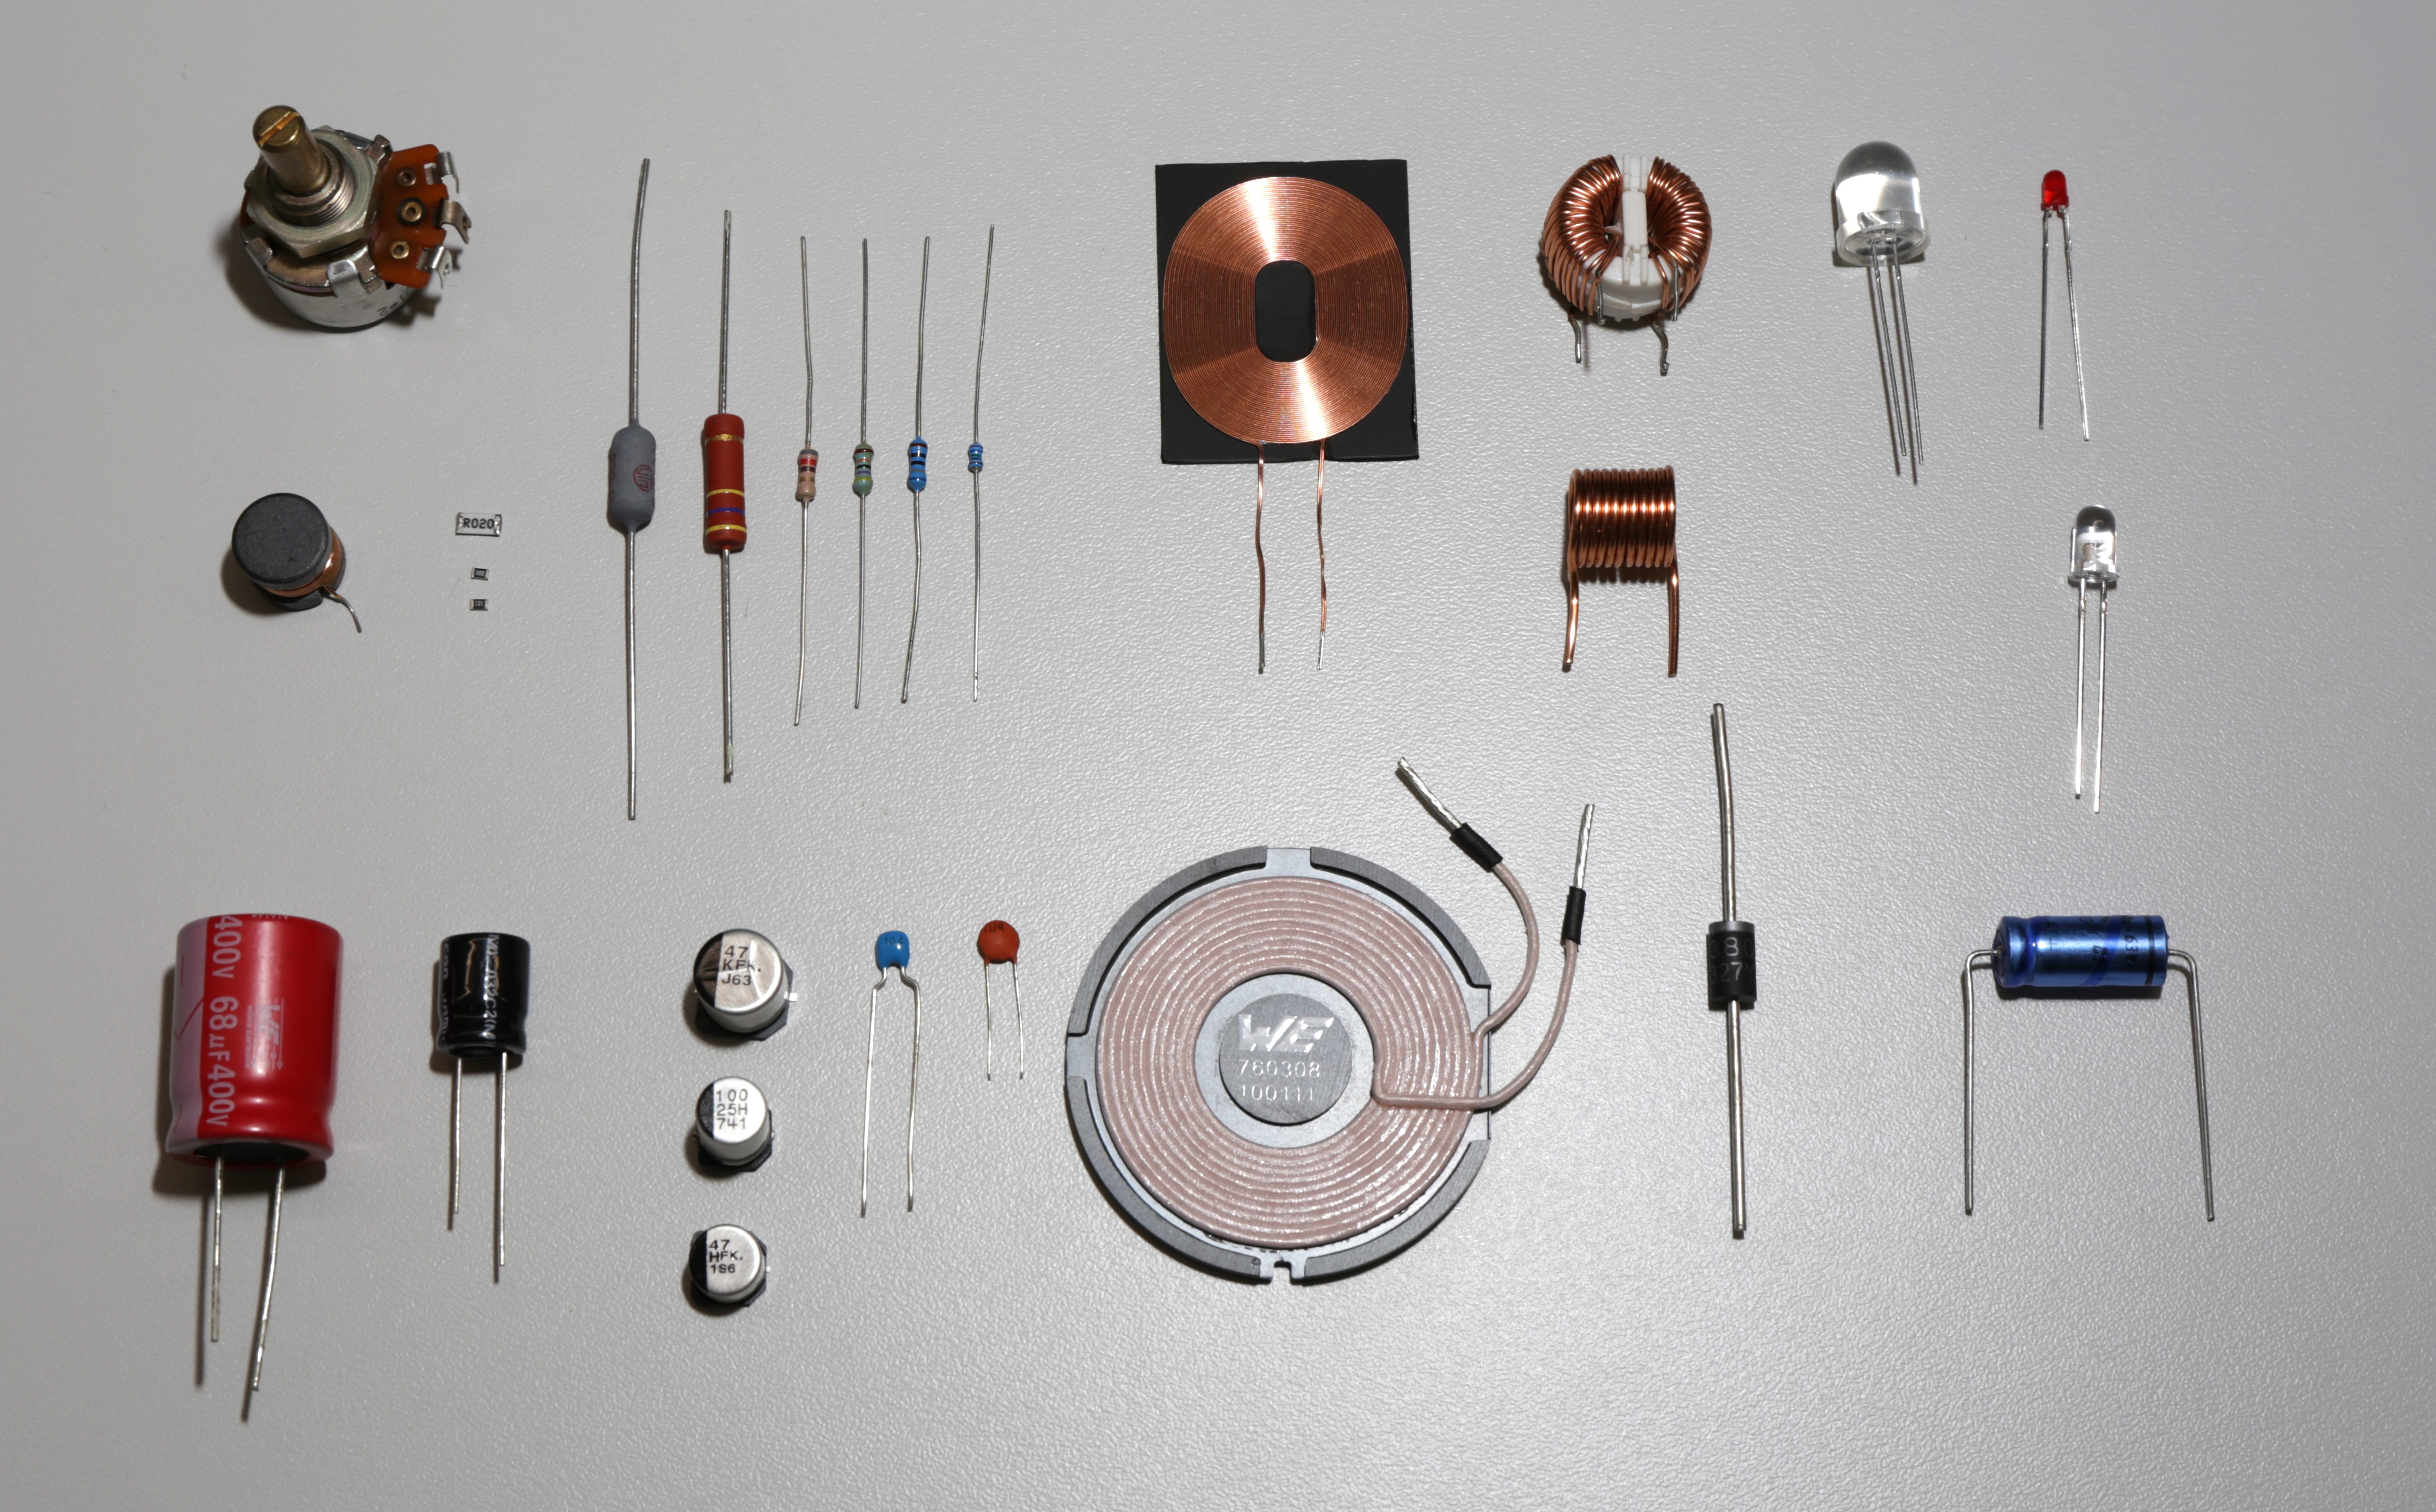
\includegraphics[width=0.65\textwidth]{ba} 
	\end{figure}
}
\speech{00_Einleitung}{1}{
Im Modul 3 beschäftigen wir uns, wie schon gesagt, mit den elektrischen Bauelementen. Auf dieser Übersichtsdarstellung sehen Sie unterschiedlichste Bauelemente. Auf einige davon, oder auf die allermeisten, werden wir nun im Folgenden eingehen.
Im linken oberen Quadrant sehen Sie unterschiedliche Ausführungen von Widerständen. Im unteren linken Quadranten sehen Sie unterschiedliche Ausführungen von Kondensatoren. Im oberen rechten Quadranten sehen Sie unterschiedliche Ausführungen von Leuchtdioden.
All diese Bauelemente werden in Schaltungen unterschiedlichster Art verwendet, damit wir die gewünschte Funktion realisieren können. Um zu verstehen, wie Bauelemente funktionieren und wie man die gewünschten Effekte bekommt, werden wir uns zuallererst mit der Leitfähigkeit und dem elektrischen Widerstand beschäftigen.
Anschließend kommen die Spannungs- und Stromquellen. Wir werden uns dann mit dem Kapazitätsbegriff und dem Kondensator als Bauteil beschäftigen und zum Schluss mit dem Induktivitätsbegriff und der Spule als Bauteil.
}


\end{frame}
%%%%%%%%%%%%%%%%%%%%%%%%%%%%%%%%%%%%%%%%%%%%% Ende - Abbildung Bauelemente %%%%%%%%%%%%%%%%%%%%%%%%%%%%%%%%%%%%

\s{% nur im Skript
Jedes dieser Bauelemente nutzt die grundlegenden Prinzipien der Elektrotechnik, um spezifische Funktionen in einem elektrischen Schaltkreis zu erfüllen. 
Durch die Kombination verschiedener Bauelemente können komplexe Schaltungen erstellt werden, die in der Lage sind, anspruchsvolle Aufgaben zu erfüllen, 
wie das Verarbeiten von Daten in einem Computer oder das Regulieren der Geschwindigkeit in einem Elektromotor.

Der Übergang von den grundlegenden physikalischen Konzepten zu den elektrischen Bauelementen ist also ein Schritt von der Theorie zur Praxis, 
der es uns ermöglicht, unser theoretisches Wissen in realen Anwendungen umzusetzen. Dieses Kapitel führt die drei grundlegenden elektrischen 
Eigenschaften von Bauelementen, sowie die Spannungs- und Stromquellen, ein.


}% nur im Skript